%; whizzy paragraph -pdf xpdf -latex ./whizzypdfptex.sh
%; whizzy-paragraph "^\\\\begin{frame}"
% latex beamer presentation.
% platex, latex-beamer でコンパイルすることを想定。

%     Tokyo Debian Meeting resources
%     Copyright (C) 2009 Junichi Uekawa
%     Copyright (C) 2009 Nobuhiro Iwamatsu

%     This program is free software; you can redistribute it and/or modify
%     it under the terms of the GNU General Public License as published by
%     the Free Software Foundation; either version 2 of the License, or
%     (at your option) any later version.

%     This program is distributed in the hope that it will be useful,
%     but WITHOUT ANY WARRANTY; without even the implied warranty of
%     MERCHANTABILITY or FITNESS FOR A PARTICULAR PURPOSE.  See the
%     GNU General Public License for more details.

%     You should have received a copy of the GNU General Public License
%     along with this program; if not, write to the Free Software
%     Foundation, Inc., 51 Franklin St, Fifth Floor, Boston, MA  02110-1301 USA

\documentclass[cjk,dvipdfmx,12pt]{beamer}
\usetheme{Tokyo}
\usepackage[english]{babel}
\usepackage{monthlypresentation}

%  preview (shell-command (concat "evince " (replace-regexp-in-string "tex$" "pdf"(buffer-file-name)) "&"))
%  presentation (shell-command (concat "xpdf -fullscreen " (replace-regexp-in-string "tex$" "pdf"(buffer-file-name)) "&"))
%  presentation (shell-command (concat "evince " (replace-regexp-in-string "tex$" "pdf"(buffer-file-name)) "&"))

%http://www.naney.org/diki/dk/hyperref.html
%日本語EUC系環境の時
\AtBeginDvi{\special{pdf:tounicode EUC-UCS2}}
%シフトJIS系環境の時
%\AtBeginDvi{\special{pdf:tounicode 90ms-RKSJ-UCS2}}

\newenvironment{commandline0}%
{\VerbatimEnvironment
  \begin{Sbox}\begin{minipage}{0.95\hsize}\begin{fontsize}{9}{9} \begin{BVerbatim}}%
{\end{BVerbatim}\end{fontsize}\end{minipage}\end{Sbox}
  \setlength{\fboxsep}{10pt}

\vspace{10pt}% skip before
\fcolorbox{dancerdarkblue}{dancerlightblue}{\TheSbox}

\vspace{6pt}% skip after
}
%end of commandline

\title{東京エリア Debian 勉強会}
\subtitle{Linuxカーネルコンフィグ変換ツール\\を作ってみた}
\author{岩松 信洋 iwamatsu@debian.or.jp\\IRC nick: iwamatsu}
\date{2009年1月17日}
\logo{
\includegraphics[width=8cm]{image200607/openlogo-light.eps}}

\begin{document}

\frame{\titlepage{}}


\emtext{冬休み}
\section{赤ちゃんが生まれました}
\begin{frame}[containsverbatim]{赤ちゃんが生まれました}
赤ちゃんが生まれたので、世話をしていました。
 \begin{center}
 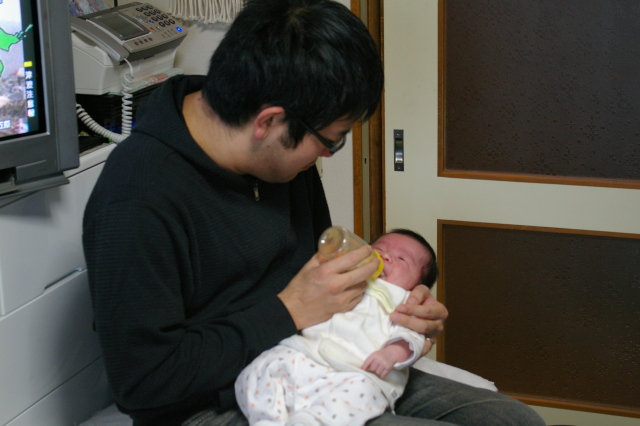
\includegraphics[scale=0.5]{image200901/baby.jpg}
 \label{fig:baby}
 \end{center}
\end{frame}

\emtext{今回作ったもの}
\section{今回作ったもの}
\begin{frame}[containsverbatim]{今回作ったもの}
\begin{center}\bfseries
システム情報を元に\\
システムに必要なカーネルモジュールを\\
組み込み指定に変換した\\
カーネルコンフィグファイルを出力する\\
スクリプト
\end{center}
\end{frame}
\begin{frame}[containsverbatim]{今回作ったもの}
\begin{center}
たいしてものではないです
\end{center}
\end{frame}


\begin{frame}{なぜこれを作ろうと思ったのか}
\begin{enumerate}
\item ひさびさにあまり使ってないマシンのカーネルコンフィグレーションをした。
\item コンフィグレーションが多すぎる。
\item 特にPCだと何を指定していいものやら。
\item 自動化できるんじゃね?
\item 自分は正規表現が苦手。正規表現の勉強のため。
\item Perlを学習する必要があった。
\item これらができて、アウトプットのできるものを作りますか。
\item 帰省の新幹線内で。
\end{enumerate}
\end{frame}

\begin{frame}{これができると}
\begin{enumerate}
\item カーネルコンフィグに悩まされずにすむ
\item 取り合えず動くカーネルはできる(はず)
\item 一般ユーザからvanilaカーネルアクセスへの敷居が下がる(かも)
\end{enumerate}
\end{frame}

\section{なぜ彼らはカーネルをリコンパイルするのか?}
\begin{frame}[containsverbatim]{}
\begin{center}
\large\bfseries
そういや、カーネルコンパイル!コンパイル!ってうるさい人たちいるよね?
\end{center}
\end{frame}

\begin{frame}[containsverbatim]
\begin{center}
\large\bfseries
なぜ彼らはカーネルをリコンパイルするのか?
\end{center}
\end{frame}

\begin{frame}{カーネルをリコンパイルする理由}
\begin{itemize}
\item カーネルハックのため。
\item カーネルBTSの深追い。
\item 最新のカーネルは新しいドライバや機能が使えるから。
\item ドライバを組み込みにして、起動の高速化。
\item ドキドキ感を味わうことができる。
\item 無駄にCPUを使いたい。(反エコ)
\end{itemize}
\end{frame}

\begin{frame}{カーネルをリコンパイルすることによるデメリット}
\begin{itemize}
\item 失敗したら動かなくなるかもしれない。
\item コンパイルにCPUリソースを食いすぎる(CPUが遅いため)。
\end{itemize}
\end{frame}

\begin{frame}{なぜ彼らはカーネルをリコンパイルするのか?}
\begin{center}
\large\bfseries
ここにいるひとたちには\\
後者なんて気にしないと思いますが。
\end{center}
\end{frame}

\emtext{内容}

\begin{frame}[containsverbatim]{必要なデータ}

\begin{itemize}
\item 使うカーネル\\
      Debianで提供しているカーネル(lenny では 2.6.26)
\item 入力するデータ
\begin{enumerate}
  \item カーネルソースコード
  \item 動いているカーネルのコンフィグファイル\\
	\url{/boot/config-2.6.26-1-xxx}
  \item システム情報
\end{enumerate}
\item 出力されるデータ\\
      システム情報を元にシステムに必要なカーネルモジュールが組み込み
      状態になっているカーネルコンフィグファイル
\end{itemize}
\end{frame}


\subsection{システム情報の取得方法}
\begin{frame}[containsverbatim]{システム情報の取得方法}
どのようにして、システム情報を取得するか。

\begin{table}[h]
 \begin{center}
 {
   \begin{tabular}{l|l} \hline
     コマンド & 内容  \\ \hline \hline
     dmidecode & BIOS からシステム情報を出力する \\
     lspci & PCI の情報を出力する \\
     lsusb & USB の情報を出力する \\
     dmesg & カーネルデバッグメッセージを出力する \\
     lsmod & ロードしてるモジュールを出力する \\
   \end{tabular}
 }
 \caption{起動しているカーネルから得られる情報}
 \label{kernel-output}
 \end{center}
\end{table}

\end{frame}

\subsection{システム情報の取得方法}
\begin{frame}[containsverbatim]{システム情報の取得方法}

今回利用したもの

\begin{table}[h]
 \begin{center}
 {
   \begin{tabular}{l|l} \hline
     コマンド & 内容  \\ \hline \hline
     lsmod & ロードしてるモジュールを出力する \\
   \end{tabular}
 }
 \caption{起動しているカーネルから得られる情報}
 \label{kernel-output}
 \end{center}
\end{table}


{\bf ロードしているモジュール=現在の Linux システムに必要なもの}
なので、わかりやすい。
\end{frame}

\emtext{簡単な流れ}

\begin{frame}{簡単な流れ}
1. データとして、
\begin{enumerate}
\item カーネルソースコードへのパス
\item 動作しているカーネルコンフィグファイル
\item lsmod の出力結果
\end{enumerate}
を指定する。

\end{frame}

\begin{frame}[containsverbatim]{簡単な流れ}
2. lsmod からロードしているドライバモジュール一覧を取得する

lsmod を実行すると、以下のような内容が出力される。
\begin{commandline0}
$ lsmod
Module                  Size  Used by
i915                   25280  2
drm                    65256  3 i915
ipv6                  235300  10
rfcomm                 28272  2
l2cap                  17248  9 rfcomm
........
\end{commandline0}
\end{frame}

\begin{frame}[containsverbatim]{簡単な流れ}

{\bf 3. ドライバモジュール名 と modinfo コマンドから ドライバモジュールのパスを取得する。}
\\

modinfo コマンドを使うと、指定したドライバモジュール名の情報を取得するこ
       とができます。-n オプションを使うと、ドライバオブジェクトファイル
       のパスが出力される。

\begin{commandline0}
$ modinfo -n i915
/lib/modules/2.6.26-1-amd64/kernel/drivers/char/drm/i915.ko
\end{commandline0}
\end{frame}

\begin{frame}[containsverbatim]{簡単な流れ}
\begin{commandline0}
$ modinfo -n i915
/lib/modules/2.6.26-1-amd64/kernel/drivers/char/drm/i915.ko
\end{commandline0}
 上の結果を例にすると、{\bf /lib/modules/2.6.26-1-amd64/kernel/} 以下と カーネルソース
 コードのパス構造は同じなため、ドライバモジュール名{\bf i915}の Makefile
 のあるパスは {\bf drivers/char/drm/Makefile} になる。

また、ドライバオブジェクトファイルは {\bf i915.ko} であることが分かる。
\end{frame}


\begin{frame}[containsverbatim]{簡単な流れ}

{\bf 4. 先で取得したMakefile へのパスとドライバオブジェクトファイル名より、
      対象になるドライバコンフィグ名を取得する。}

      ドライバオブジェクトファイル(i915.ko)とドライバモジュール名(i915)
      は必ずしも一致するとは限らないので、ドライバモジュール名を使って、
      ドライバコンフィグ名を検索する。(例えば snd\_hda\_intel)

\begin{commandline0}
.....
obj-$(CONFIG_DRM_I830)  += i830.o
obj-$(CONFIG_DRM_I915)  += i915.o <- これ
obj-$(CONFIG_DRM_SIS)   += sis.o
.....
\end{commandline0}
\end{frame}

\begin{frame}[containsverbatim]{簡単な流れ}

{\bf 5. 取得したドライバコンフィグ名を保存する。}
\end{frame}

\begin{frame}[containsverbatim]{簡単な流れ}

{\bf 6. 動作しているカーネルコンフィグファイルのドライバコンフィグを書き換える。}

正規表現を使って書き換えると、以下のようになる。
{\bf m} はモジュールを意味し、{\bf y} は組み込みを意味する。

変更前
\begin{commandline0}
....
CONFIG_DRM_I830=m
CONFIG_DRM_I915=m
CONFIG_DRM_MGA=m
....
\end{commandline0}

変更後
\begin{commandline0}
....
CONFIG_DRM_I830=m
CONFIG_DRM_I915=y <- 書き換え
CONFIG_DRM_MGA=m
....
\end{commandline0}
\end{frame}

\begin{frame}[containsverbatim]{簡単な流れ}

{\bf 7. 変更したものをファイルに出力する。}

\end{frame}


\emtext{実際に使ってみる}

\begin{frame}[containsverbatim]{ 実際に使ってみる}
\begin{commandline0}
$ moge -h
moge - Script to Kernel Module Enabler from lsmod command output

Copyright (C) 2008,2009 Nobuhiro Iwamatsu <iwamatsu@nigauri.org>
Usage: moge [options]
	-c, --configfile <file>   Kernel config file name
	-k, --kernel              Kernel source path
	-o, --output <file>       outout file
	-l, --lsmod               lsmod command output file
	-h, --help                display this help screen and exit
	-v, --version             show the version and exit

By Nobuhiro Iwamatsu <iwmatsu@nigauri.org>
$ moge -o sage -c config-2.6.26-1-686 -l lsmod.list -k \
                         /usr/src/linux-2.6-2.6.26/
\end{commandline0}
\end{frame}


\emtext{作成されたコンフィグファイルを使ってカーネルをコンパイルする}

\begin{frame}[containsverbatim]{カーネルコンパイルをする}
作成されたコンフィグファイルを使ってカーネルをコンパイルしてみる。

\begin{commandline0}
$ sudo apt-get update
$ sudo apt-get install linux-source-2.6.26 kernel-package
$ cd /usr/src/linux-source-2.6.26
$ make oldconfig
$ fakeroot make-kpkg --revision=yourpc00 kernel_image kenrel_header
$ ls ../
linux-image-2.6.26_yourpc00_i386.deb
linux-headers-2.6.26_yourpc00_i386.deb
.......
\end{commandline0}
\end{frame}

\section{変更結果}
\begin{frame}[containsverbatim]{lsmodの結果}

eeePC で試してみて、どれぐらい変わったのか調べてみた。

変更前 61モジュール
\begin{commandline0}
$ lsmod
Module                  Size  Used by
i915                   25280  2
drm                    65256  3 i915
ipv6                  235300  10
rfcomm                 28272  2

......

ide_core               96168  1 ide_pci_generic
ehci_hcd               28428  0
uhci_hcd               18672  0
usbcore               118160  5 uvcvideo,usb_storage,ehci_hcd,
uhci_hcd
thermal                15228  0
processor              32576  2 thermal
fan                     4164  0
thermal_sys            10856  4 video,thermal,processor,fan
\end{commandline0}
\end{frame}

\begin{frame}[containsverbatim]{lsmodの結果}

 変更後 0モジュール
\begin{commandline0}
$ lsmod
Module                  Size  Used by
\end{commandline0}

\end{frame}

\begin{frame}{bootchart}

{\bf bootchartでどれぐらい起動が速くなったか、調べてみました。}

\end{frame}

\begin{frame}{bootchart 変更前}
\begin{figure}
 \begin{center}
 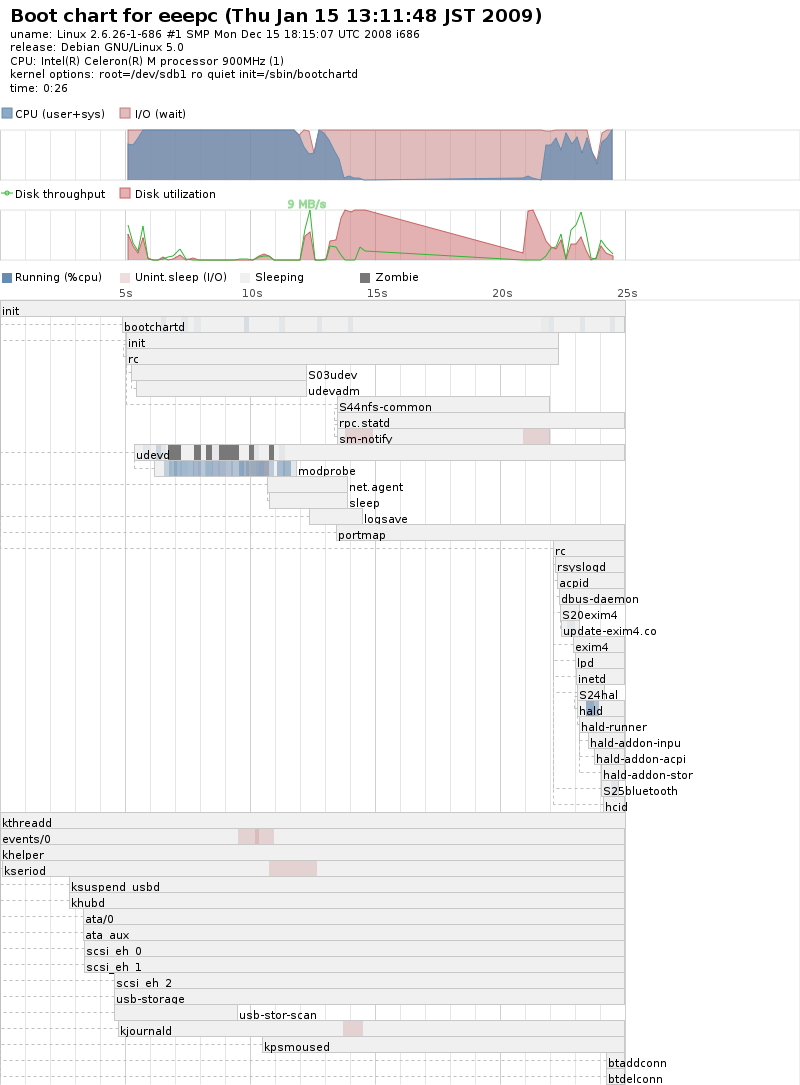
\includegraphics[scale=1.0]{image200901/bootchart-eeepc.png}
 \caption{変更前のbootchart}
 \label{fig:bootchart-eeepc}
 \end{center}
\end{figure}

\end{frame}

\begin{frame}{bootchart 変更後}
\begin{figure}
 \begin{center}
 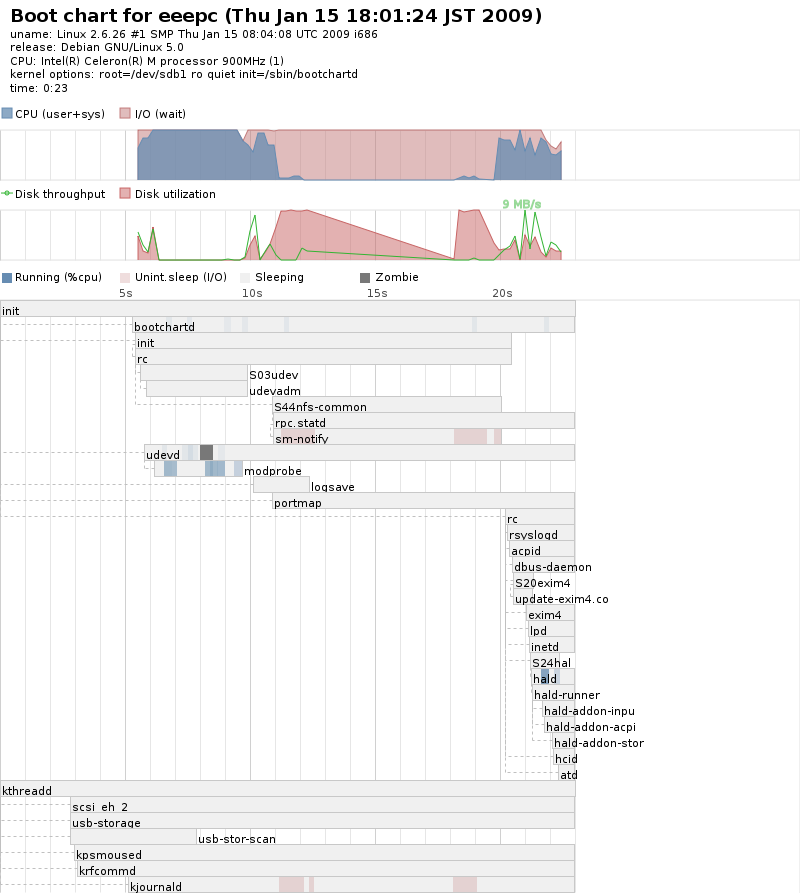
\includegraphics[scale=1.0]{image200901/bootchart-eeepc-new.png}
 \caption{変更後のbootchart}
 \label{fig:bootchart-eeepc-new}
 \end{center}
\end{figure}

\end{frame}

\begin{frame}{モジュールロード部分}
\begin{figure}
 \begin{center}
 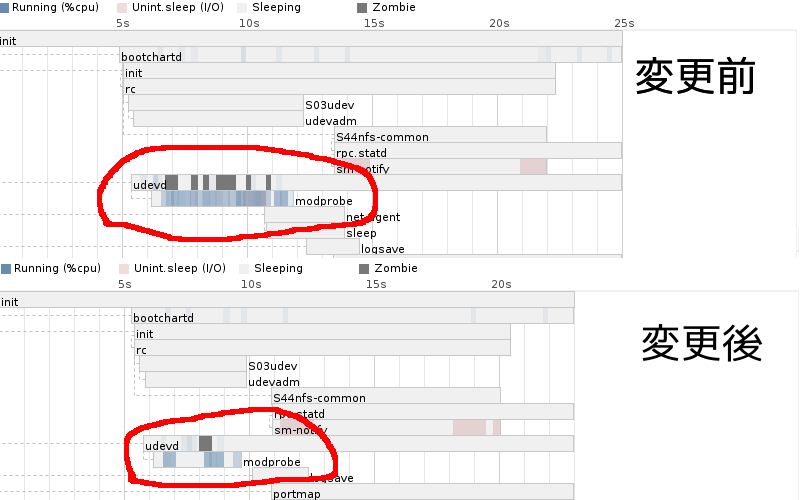
\includegraphics[scale=0.6]{image200901/bootchart-eeepc-merge.png}
 \caption{モジュールロード部分}
 \label{fig:bootchart-eeepc-merge}
 \end{center}
\end{figure}

\end{frame}


\section{今後の予定}
\begin{frame}{今後の予定}
\begin{enumerate}
 \item make-kpkg に入れる?
 \item パッケージ化?
 \item カーネルコンパイルWebサービスの提供?
 \item ドライバオブジェクトファイルとドライバモジュール名が一致しないやつを直す。
\end{enumerate}
\end{frame}


\end{document}

%;;; Local Variables: ***
%;;; outline-regexp: "\\([ 	]*\\\\\\(documentstyle\\|documentclass\\|emtext\\|section\\|begin{frame}\\)\\*?[ 	]*[[{]\\|[]+\\)" ***
%;;; End: ***
